\documentclass[./main]{subfiles} % これを最初に書く


% ここにnewtheorem,newenvironment,defなどを書く

\begin{document} %ここから文章を始める

%\newtheorem{theo}{定理}
\newtheorem{maskdefi}{定義}
\newtheorem{rem}{注意}

\Chapter{四次元立方体の描き方(マスク)} 
% 章だてはSection,Subsection,Subsubsectionで行う
\Section{四次元立方体を描いてみよう}

四次元の立体がどのような形状をしているのか,ほとんどの方は正確にイメージすることができないと思います.それは我々が手に取って観察できる立体が,三次元より低い次元のものしかないからです.

では,我々は四次以上の次元の様子を知ることはできないのでしょうか? いいえ,そんなことはありません.高次元のように目に見えないものの様子を調べることができる,それもまた数学の力の一つだと私は考えます.

今回紹介する``四次元立方体の描き方''は,その中のほんの一例です.

早速,描き方を解説していきます.

\Subsection{1}

普通の三次元の立方体を描きます.(これは普段あなたが描いているもので問題ありません.図は一例です.)

\begin{figure}[h]
\begin{center}
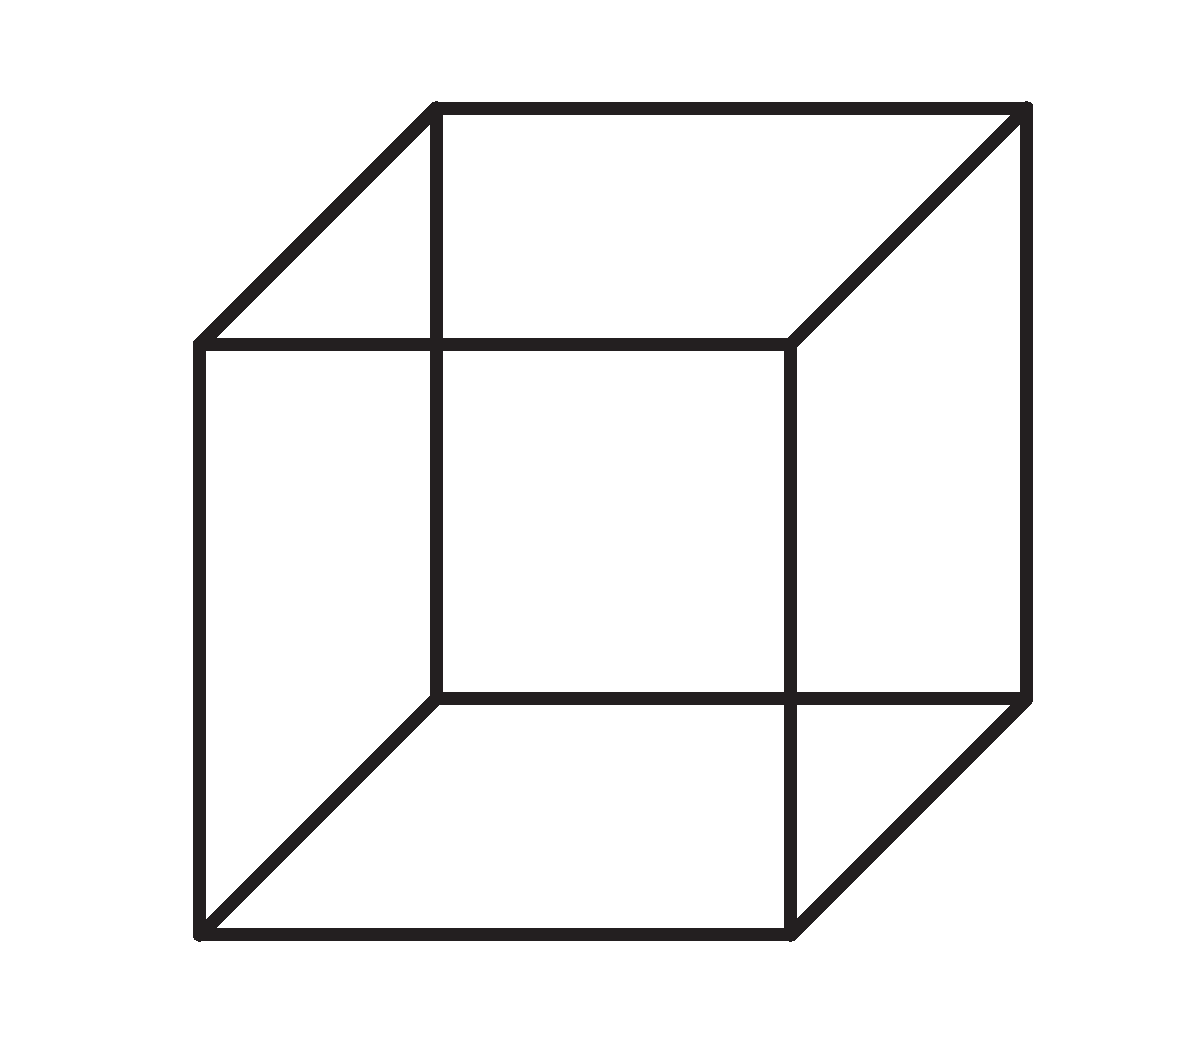
\includegraphics[width=30mm]{mask_rittai1.eps}
\end{center}
\end{figure}

\Subsection{2}

同じ三次元の立方体を,ずらした位置にもう一つ描きます.

\begin{figure}[h]
\begin{center}
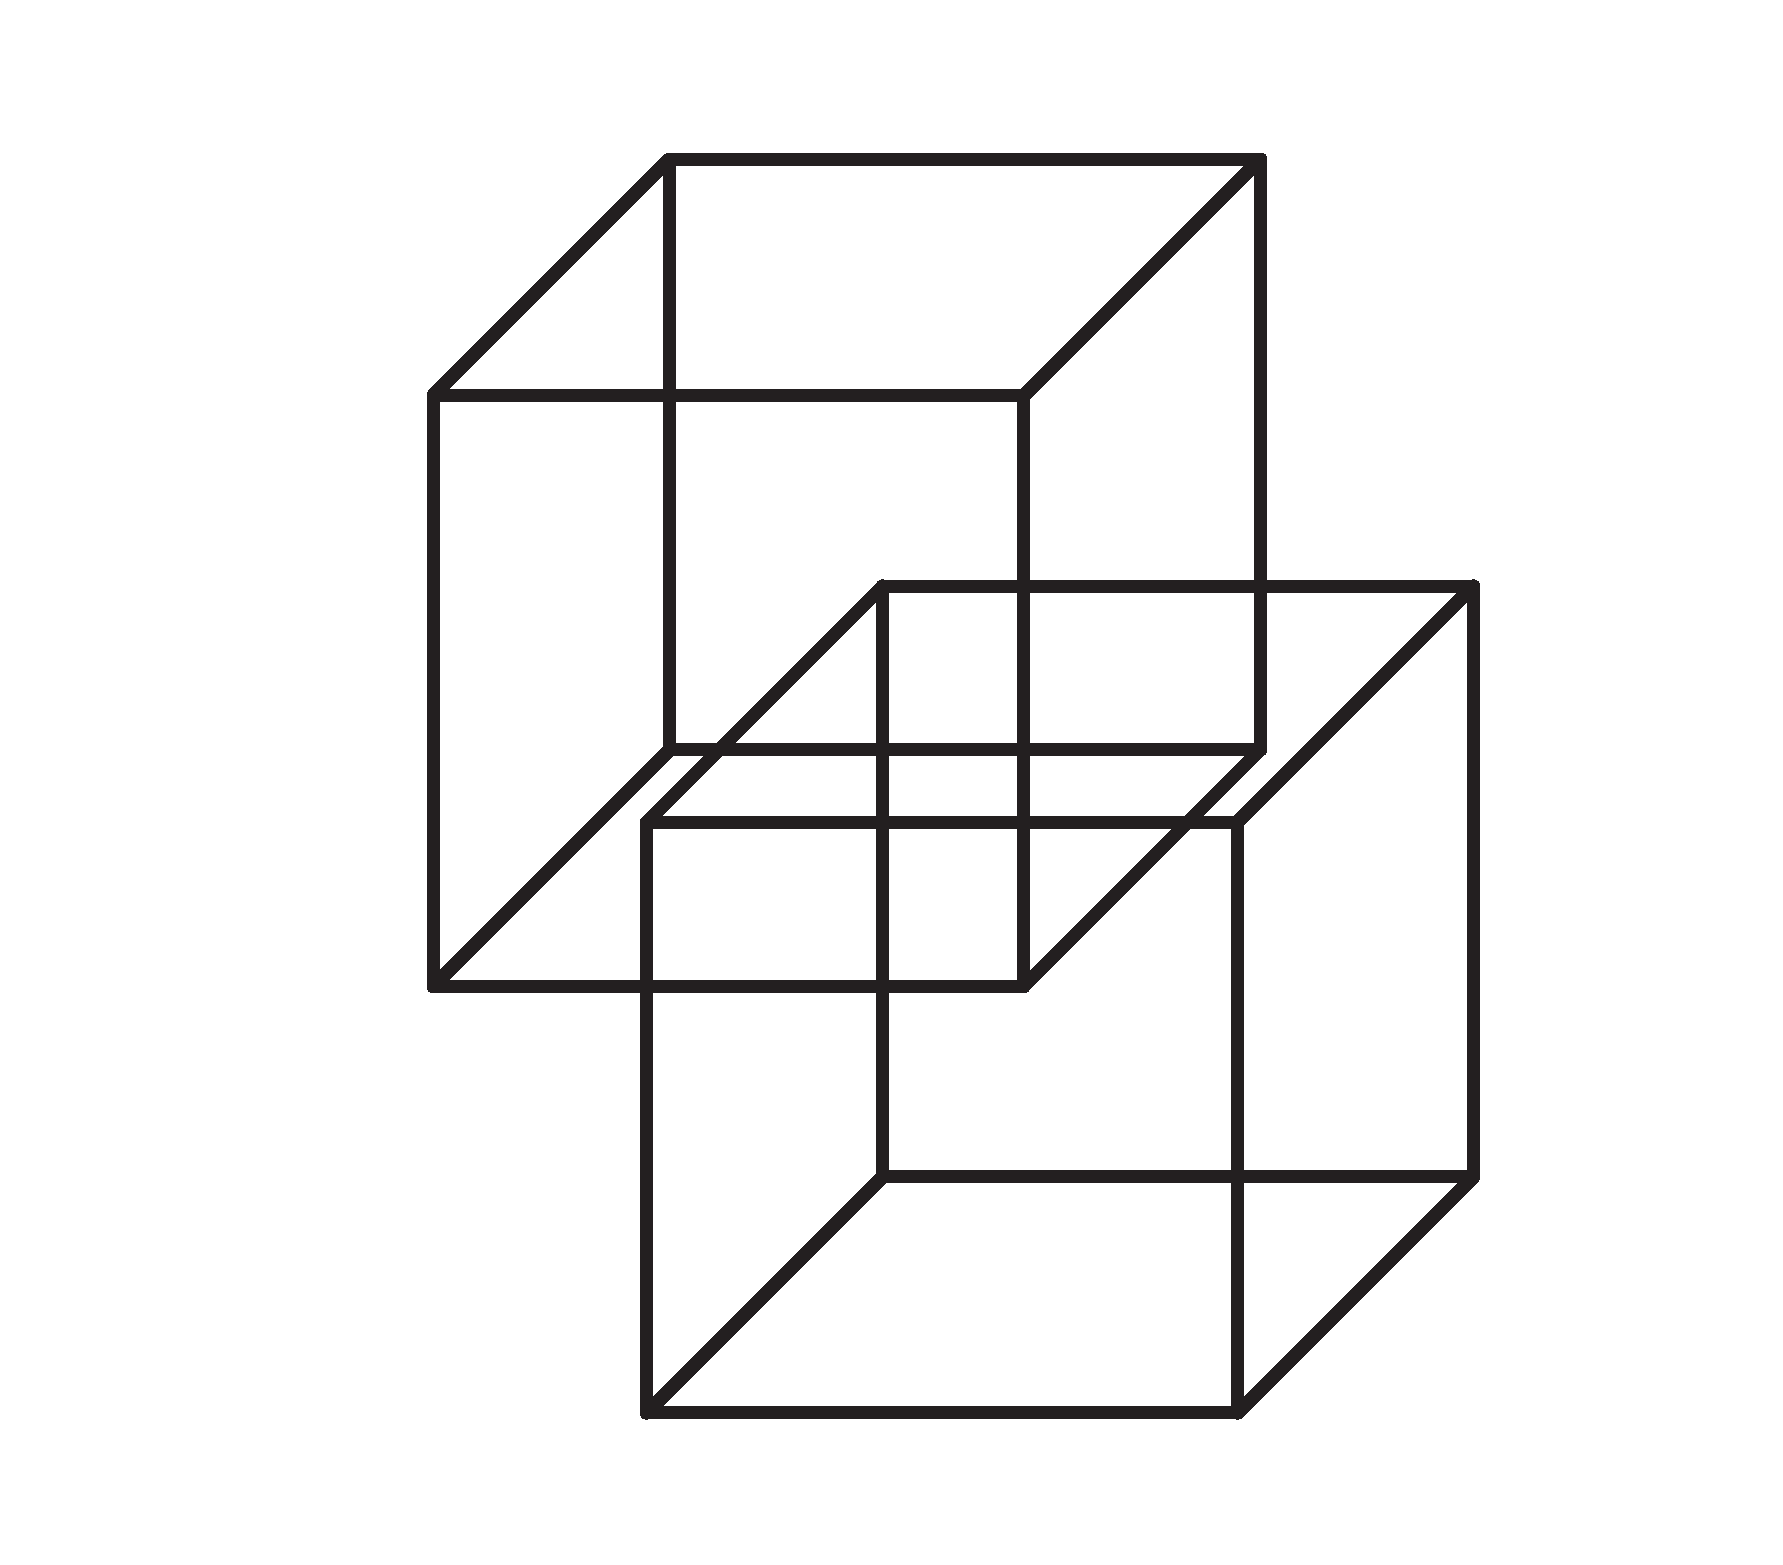
\includegraphics[width=48mm]{mask_rittai2.eps}
\end{center}
\end{figure}

\Subsection{3}

頂点を線分で結びます.

\begin{figure}[h]
\begin{center}
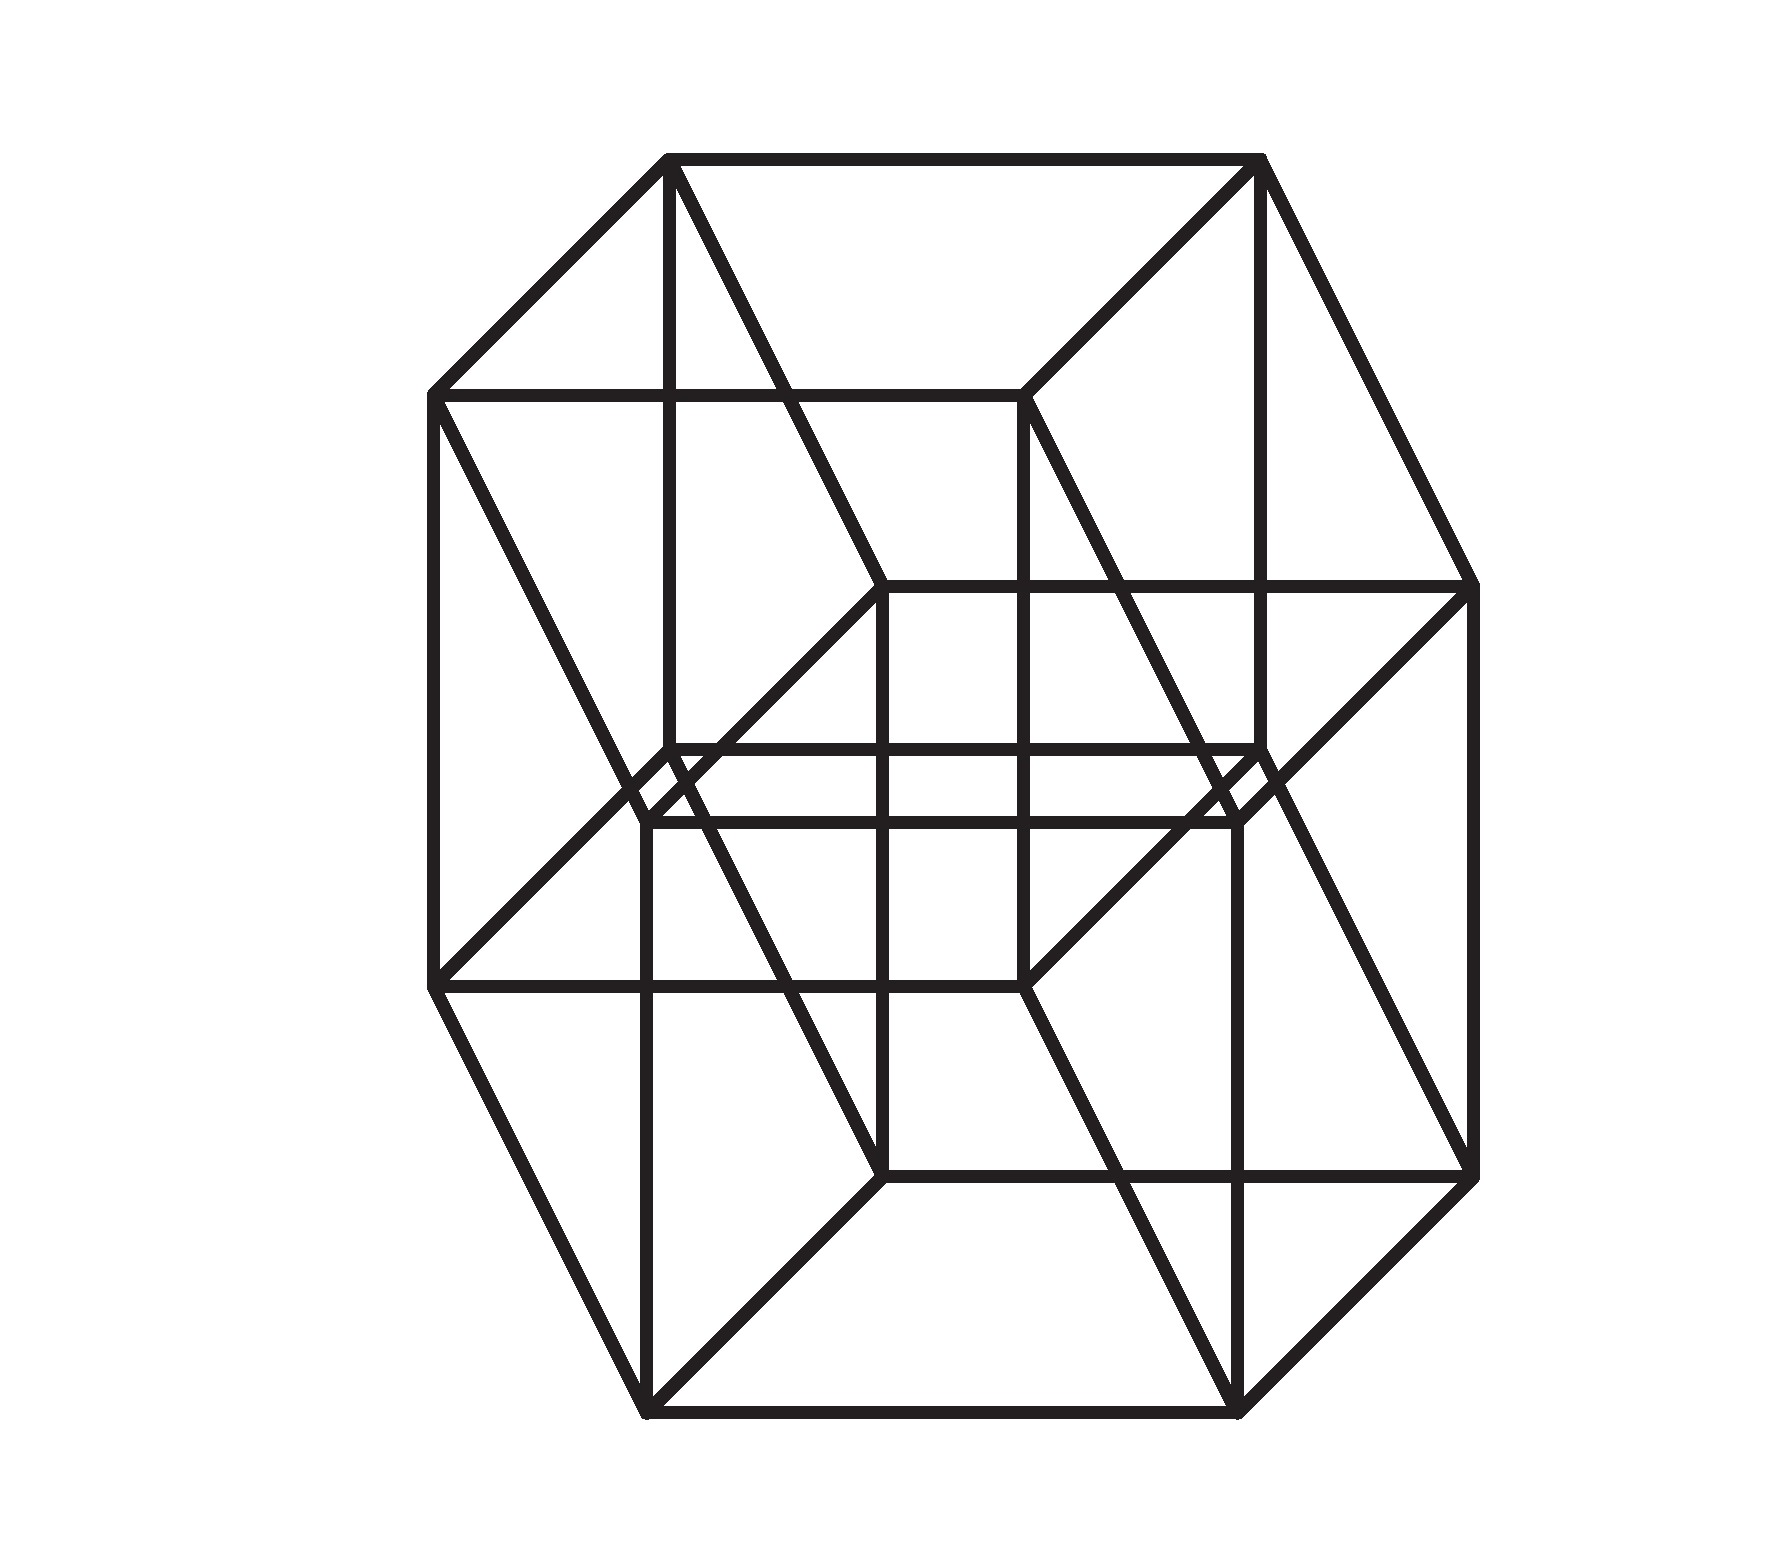
\includegraphics[width=48mm]{mask_rittai3.eps}
\end{center}
\end{figure}

これで完成です.

\Section{前ページで何をしていたのか}

前ページで四次元立方体の具体的な描き方の一例を紹介しました.それでもう満足という方は,さっさと次の記事に行っていただいて構いません.この章は先程の描き方でどうして四次元立方体を描けるのか,それを数学的に正当化するのを目的としています.

また,この章は大学一年生レベルの線型代数の知識を前提としています.

\maskdefi [$n$次元立方体]

$\mathbb{R}^n$ の部分集合 $M$ が,以下の条件を満たすとき,$M$を$n$次元立方体と呼ぶ.

\[
^\exists A \in O(n) , ^\exists b \in \mathbb{R}^n , ^\exists a \in \mathbb{R}_{>0} \quad s.t. \quad M = A ([0,a]^n) + b
\]

ただし,$O(n)$は$n$次直交行列の集合で,$[0,a]^n$は閉区間$[0,a]$の$n$個の直積である.

\rem

上の定義は,$n$次元立方体が,$[0,1]^n$を$\mathbb{R}^n$内で回転したり,平行移動をしたり,拡大縮小をして得られる図形であることを言っている.

\rem
上の理由で,今後は$n$次元立方体は全て$[0,1]^n$として考えることにする.

\maskdefi [頂点]

集合$\{0,1\} ^n \subset \mathbb{R}^n$の元を$n$次元立方体の{\gt 頂点}と呼ぶ.

\maskdefi[辺]
$n$次元立方体の異なる二つの頂点を結んだ線分のうち,長さが$1$になる線分のことを,$n$次元立方体の{\gt 辺}と呼ぶ.

\rem
上の頂点,辺の定義は$n$次元立方体に特化した定義であり,一般の$n$次元の立体に適応できるものではない.今回は,これを紙面に図示するという観点から,イメージしやすいようにこの定義を採用している.

\maskdefi [$n$次元立方体を描く]

$n$次元立方体を描くとは,次の操作のことを指す.

どの異なる二つのベクトルをとっても,線型独立となるような$\mathbb{R}^2$のベクトルの組$v_1, v_2 , \ldots , v_n$を一つ固定する.$\mathbb{R}^n$の標準基底$e_1 , e_2 , \ldots , e_n$を,$v_1,v_2 \ldots ,v_n$にそれぞれうつす線型写像$f \colon \mathbb{R}^n \rightarrow \mathbb{R}^2$を考え,それによる$n$次元立方体の頂点と辺の像を$2$次元平面に図示する.

\rem
上の定義を雑に説明すると,$n$次元立方体を描くとは,$\mathbb{R}^n$の標準基底を$\mathbb{R}^2$上のいい感じなベクトルの組にうつしたときの像を描くことである.

\rem

上の定義は前ページの描き方は含んでいるが,$n$次元立方体をどう描くかは個人の自由である.当然,上の定義以外で意味を持つ描き方もこの世には存在している.よって,もし``$4$次元立方体''とGoogleで検索して上の定義に当てはまらない図が出てきても,筆者を責めてはいけない.決して責めてはいけない.

\Subsection{まとめ}
以上の定義により,前ページの描き方が四次元立方体を描いたものだといいうことがご理解いただけたかと思います.三次元立方体をずらした向きが,ベクトル$v_4$に対応しているのです.

\Section{おまけ}
せっかく$n$次元立方体の描き方を定義したのだから,もっと高次元の立方体を見てみたい,という欲張りな人のためにこの章を用意した.結論から述べると,$n$次元立方体の辺は$n2^{n-1}$本あるので,計算量のオーダーはは$n2^n$となり,すぐに{\rm CPU}が逝く.また,図を見ればわかるがぐっちょぐちょなので,まるでよくわからん.もっともっと高次元が欲しい欲しがりは,自分の手を動かしなさい.ベクトルは$e^{\frac{2\pi i}{n}}$の組を取り,使用ソフトは{\rm Geogebra}である.

\begin{figure}[h]
\begin{center}
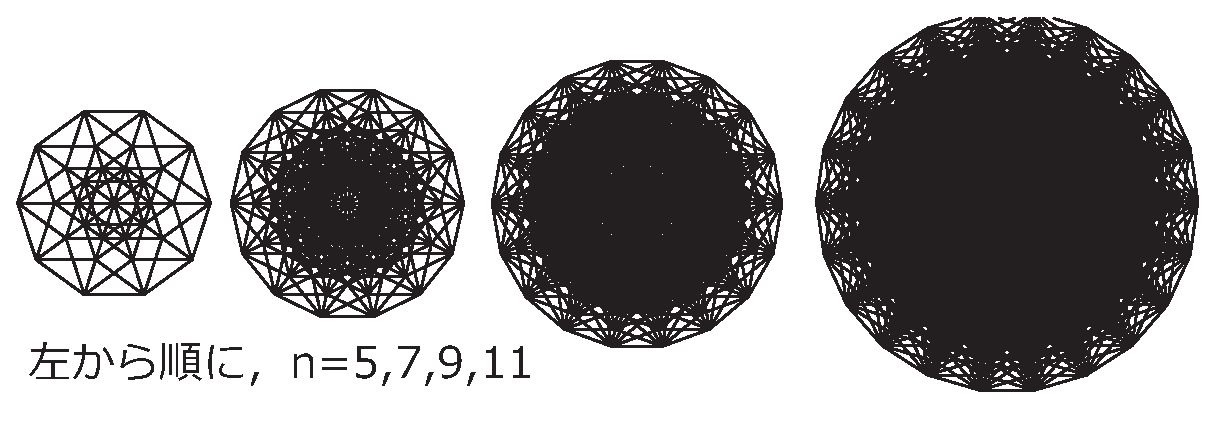
\includegraphics[width=80mm]{mask_rittai4.eps}
\end{center}
\end{figure}


\end{document}

%\begin{thebibliography}{9}
%\item Hull, J. C. (2014), Options, Futures, and Other Derivatives, 9th edition (Upper Saddle River, NJ: Prentice Hall).
%\end{thebibliography}
